\chapter{Mathematical Tools}
\label{chapter1}

\section{An overview of Differential Geometry}
We shall begin with a recall of very well known definitions in order to introduce the basic geometrical objects which are used in the text.\\

A \textbf{manifold} is essentially a space that is locally similar to $\mR^n$. To define it we use the concepts of \textbf{topological space} and of \textbf{homeomorphism}.
\begin{definition}[\textbf{Topological Space}]
	A set $\mathrm{X}$ together with a family $\mathcal{T}$ (\textbf{topology}) of subset of $\mathrm{X}$ is called a \textbf{topological space} if the following are satisfied:
	\begin{enumerate}[label=\alph*. ]
		\item $\emptyset,\mathrm{X}\in\mathcal{T}$,
		\item for all $U$ and $V\in\mathcal{T}$, $U\cap V\in\mathcal{T}$,
		\item for any index set $A$, if $U_i\in\mathcal{T}$ for all $i\in A$, $\ds \bigcup_{i\in A} U_i\in\mathcal{T}$.
	\end{enumerate}
	A set in $\mathcal{T}$ is called \textbf{open}. If a point $p$ is in an open $U$, we call $U$ a \textbf{neighborhood} of $p$.
\end{definition}

\begin{definition}[\textbf{Continuity and homomorphism}]
	Let $\mathrm{X}$ and $\mathrm{Y}$ be two topological spaces. A function $f:\mathrm{X}\to\mathrm{Y}$ is \textbf{continuous} if for any open set $U$ of $\mathrm{Y}$, the preimage $f^{-1}(U)$ is an open set of $\mathrm{X}$.\\
	A continuous and bijective map $\varphi:\mathrm{X}\to\mathrm{Y}$ is an \textbf{homomorphism} if $\varphi^{-1}:\mathrm{Y}\to\mathrm{X}$ is also continuous.
\end{definition}
As in vectorial space, we can talk about \textbf{basis} of topological spaces. A subset $\mathcal{B}\subset\mathcal{T}$ is a basis if any open can be expressed as union of elements of $\mathcal{B}$.\\
A topology is \textbf{Haussdorf} if for any two distinct points $p,q\in\mathrm{X}$, there exist two open neighborhoods $U$ of $p$ and $V$ of $q$ such that $U\cap V=\emptyset$.\\


A topological space $\mathrm{X}$ is called \textbf{compact} if each of its open covers has a finite subcover, i.e. for any collection $\{U_i\}_{i\in A}$, (where $A$ is a set of indexes) such that $$\mathrm{X}\subseteq\bigcup_{i\in A}U_i,$$ there is a finite subset $A'$ of $A$ such that $$ \mathrm{X}\subseteq\bigcup_{i\in A'}U_i.$$

We are now ready to introduce the concept of \textbf{manifold}.
\begin{definition}
	An $n$-dimensional \textbf{manifold} $\mathrm{M}$ is a topological Haussdorf space (with a countable basis) that is locally homeomorphic to $\mR^n$, i.e. for every $p\in\mM$ there exists an open neighbourhood $U$ of $p$ and a homeomorphism $$\varphi:U\to\varphi(U)$$ such that $\varphi(U)$ is an open subset of $\mR^n$.
\end{definition}
	
	Such a homeomorphism is called a \textbf{(local) coordinate chart} of $\mM$. An \textbf{atlas} of $\mM$ is a family $\{U_i,\varphi_i\}_{i\in A}$ of local charts together with an open covering of $\mM$, i.e. $ \bigcup_{i\in A}U_i=\mM$.

	
\begin{figure}[h]
	\centering
	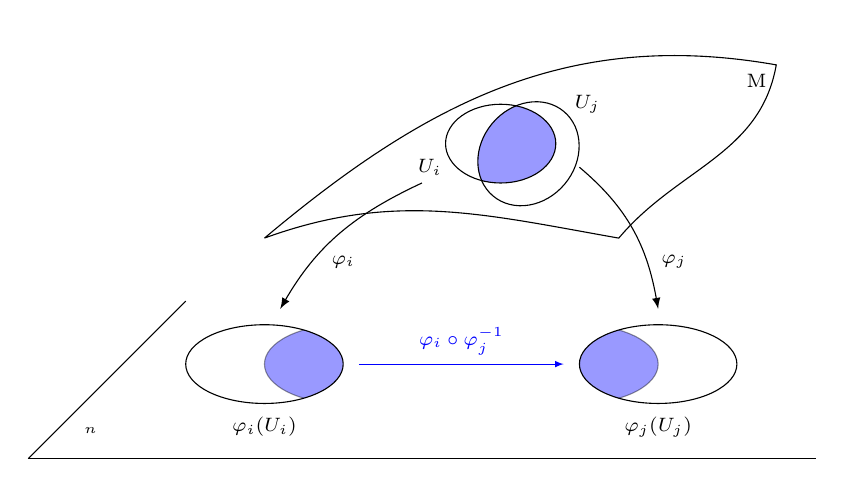
\begin{tikzpicture}[scale=1]
	\tikzstyle{every node}=[font=\scriptsize]
	\draw (0,0)  -- (10,0);
	\draw (0,0) -- (2,2);
	\node at (0.8,0.3) {$\mR^n$};
	
	\begin{scope}
	\clip (3,1.2) ellipse (1cm and 0.5cm);
	\draw [draw=black, fill=blue, opacity=0.4] (4,1.2) ellipse (1cm and 0.5cm);
	\end{scope}
	
	\begin{scope}
	\clip (8,1.2) ellipse (1cm and 0.5cm);
	\draw [draw=black, fill=blue, opacity=0.4] (7,1.2) ellipse (1cm and 0.5cm);
	\end{scope}
	
	\draw (3,1.2) ellipse (1cm and 0.5cm);
	\node at (3,0.4) {$\varphi_i(U_i) $};
	
	
	\draw [-latex] (5,3.5) to[out=-155,in=60] (3.2,1.9) node at (4,2.5) {$\varphi_i$};
	
	
	\draw (8,1.2) ellipse (1cm and 0.5cm);
	\node at (8,0.4) {$\varphi_j(U_j) $};
	
	\draw [-latex] (7,3.7) to[out=-40,in=100] (8,1.9) node at (8.2,2.5) {$\varphi_j$};
	
	
	\draw [ultra thin,-latex, color=blue] (4.2, 1.2) -- (6.8,1.2) node [pos=0.5,above] {$\varphi_i\circ\varphi_j^{-1}$};
	\draw (3,2.8) to[out=40,in=170] (9.5,5) node[below left] {$\mathrm{M}$} to[out=-100,in=50]  (7.5,2.8) to[out=170,in=20] (3,2.8);
	
	\node at (5.1,3.7) {$U_i$};
	\node at (7.1,4.5) {$U_j$};
	
	
	\begin{scope}
	\clip (6,4) ellipse (0.7cm and 0.5cm);
	\fill[blue, opacity=0.4, rotate around={-40:(6.2,4)}] (6.4,4) ellipse (0.6cm and 0.7cm);
	\end{scope}
	\draw [thin] (6,4) ellipse (0.7cm and 0.5cm);
	\draw [thin, rotate around={-40:(6.2,4)}] (6.4,4) ellipse (0.6cm and 0.7cm);
	
	\end{tikzpicture}
	\label{fig:atlas}
	\caption{A differentiable atlas on a manifold $\mM$.}
\end{figure}

\begin{definition}
	A \textbf{differentiable atlas} of a manifold $\mM$ is an atlas $\{U_i,\varphi_i\}_{i\in A}$ such that the function
	$$\textcolor{blue}{\varphi_i\circ\varphi_j^{-1}}:\varphi_j(U_i\cap U_j)\to\varphi_j(U_i\cap U_j),$$
	called \textbf{chart transition}, is differentiable (of class $C^\infty$) for any $i,j\in A$ such that $U_i\cap U_j\neq \emptyset$.
\end{definition}


	With this definition, such chart transitions are \textbf{diffeomorphisms} because you can always interchange the indexes $i$ and $j$.\\



We are only interested in \textbf{differentiable} (or \textbf{smooth}) \textbf{manifolds}, which are manifolds together with a maximal differentiable atlas. Here maximality of the atlas means that if $\varphi$ is a chart of $\mM$ and $\{U_i,\varphi_i\}_{i\in A}$ is a differentiable atlas, then $\varphi$ itself also belongs to $\{U_i,\varphi_i\}_{i\in A}$. We call a differentiable manifold with an atlas for which all chart transitions have positive jacobian determinant an \textbf{orientable manifold}.
\begin{notation}
	For now on the word \textbf{manifold} will always mean \textbf{differentiable manifold}.
\end{notation}


\begin{definition}[\textbf{Submanifold}]
	Let $n\leq m$. An $n$-dimensional \textbf{submanifold} $\mathrm{N}$ of an $m$-dimensional manifold $\mM$ is a nonempty subset $\mathrm{N}$ of $\mM$ such that for every point $q\in\mathrm{N}$ there exists a local chart $\{U,\varphi\}$ of $\mM$ about $q$ with
	$$\varphi(U\cap \mathrm{N})=\varphi(U)\cap(\mR^n\times\{0\})\subset\mR^m.$$ In case $n=m-1$ we call $\mathrm{N}$ an \textbf{hypersurface} of $\mM$.
\end{definition}

\begin{example}
	If $\mM$ and $\mathrm{N}$ are manifolds, the cartesian product $\mM\times\mathrm{N}$ is also a manifold. If $\{U_i,\varphi_i\}_{i\in A}$ is an differentiable atlas for $\mM$ and $\{V_j,\psi_j\}_{j\in B}$ ia an atlas for $\mathrm{N}$, then $\big\{U_i\times V_j,(\varphi_i,\psi_j)\big\}_{(i,j)\in A\times B}$ is a differentiable atlas for $\mM\times\mathrm{N}$.
\end{example}

As in the euclidean case, we have the concept of \textbf{differentiable} map between manifolds:
\begin{figure}[h]
	\centering
	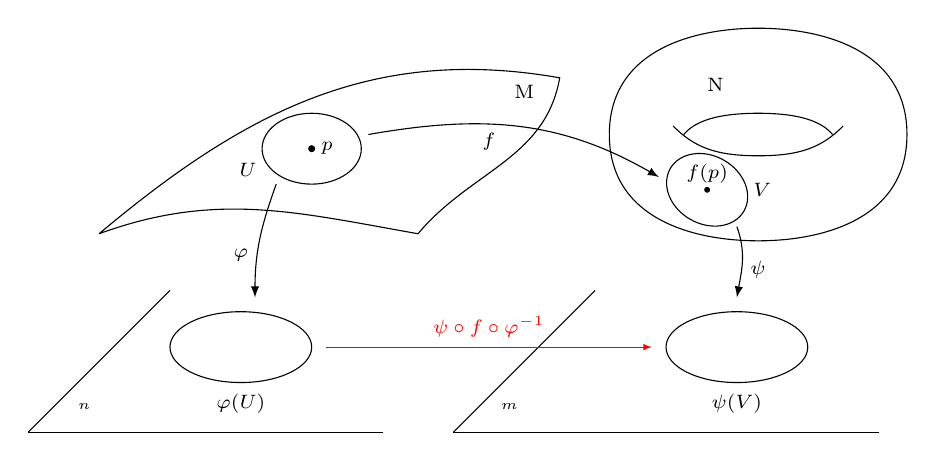
\begin{tikzpicture}[scale=0.9]
	\tikzstyle{every node}=[font=\scriptsize]
	\draw (0,0)  -- (5,0);
	\draw (0,0) -- (2,2);
	\node at (0.8,0.3) {$\mR^n$};
	\draw (6,0)  -- (12,0);
	\draw (6,0) -- (8,2);
	\node at (6.8,0.3) {$\mR^m$};
	
	
	
	
	\draw [thin] (3,1.2) ellipse (1cm and 0.5cm);
	\node at (3,0.4) {$\varphi(U) $};
	
	
	\draw [-latex] (3.5,3.5) to[out=-110,in=90] (3.2,1.9) node at (3,2.5) {$\varphi$};
	
	
	\draw [thin] (10,1.2) ellipse (1cm and 0.5cm);
	\node at (10,0.4) {$\psi(V) $};
	
	\draw [-latex] (10,2.9) to[out=-70,in=80] (10,1.9) node at (10.3,2.3) {$\psi$};
	
	\draw [-latex] (4.8,4.2) to[out=10,in=150] (8.9,3.6);
	\node at (6.5,4.1) {$f$};
	
	
	\draw [ultra thin,-latex, color=red] (4.2, 1.2) -- (8.8,1.2) node [pos=0.5,above] {$\psi\circ f\circ\varphi^{-1}$};
	
	
	\draw (1,2.8) to[out=40,in=170] (7.5,5) node at (7,4.8) {$\mathrm{M}$} to[out=-100,in=50]  (5.5,2.8) to[out=170,in=20] (1,2.8);
	
	\node at (3.1,3.7) {$U$};
	
	\draw [thin] (4,4) ellipse (0.7cm and 0.5cm);
	\fill [black] (4,4) circle (0.05cm) node [right] {$p$};
	
	\node at (9.7,4.9) {$\mathrm{N}$};
	
	\begin{scope}[shift={(10.3,4.2)},scale=0.6]
	
	
	
	\draw (-3.5,0) .. controls (-3.5,2) and (-1.5,2.5) .. (0,2.5);
	\draw[xscale=-1] (-3.5,0) .. controls (-3.5,2) and (-1.5,2.5) .. (0,2.5);
	\draw[rotate=180] (-3.5,0) .. controls (-3.5,2) and (-1.5,2.5) .. (0,2.5);
	\draw[yscale=-1] (-3.5,0) .. controls (-3.5,2) and (-1.5,2.5) .. (0,2.5);
	
	\draw (-2,.2) .. controls (-1.5,-0.3) and (-1,-0.5) .. (0,-.5) .. controls (1,-0.5) and (1.5,-0.3) .. (2,0.2);
	
	\draw (-1.75,0) .. controls (-1.5,0.3) and (-1,0.5) .. (0,.5) .. controls (1,0.5) and (1.5,0.3) .. (1.75,0);
	\draw [thin, rotate around={-30:(-1.2,-1.3)}] (-1.2,-1.3) ellipse (1cm and 0.8cm);
	\fill [black] (-1.2,-1.3) circle (0.07cm) node at (-1.2,-0.93) {$f(p)$};
	\node at (0.1,-1.3) {$V$};
	\end{scope}
	
	
	
	
	\end{tikzpicture}
	\label{fig:diffmap}
	\caption{The concept of differentiable map $f$ between manifolds $\mM$ and $\mathrm{N}$.}
\end{figure}

\begin{definition}
	A continuous map $f:\mM\to\mathrm{N}$ between manifolds $\mM$ and $\mathrm{N}$ is \textbf{differentiable} in $p\in\mM$ if there exist local charts $\{U,\varphi\}$ and $\{V,\psi\}$ about $p$ in $\mM$ and about $f(p)$ in $\mathrm{N}$ respectively, such that $f(U)\subset V$ and
	$$ \textcolor{red}{\psi\circ f\circ \varphi^{-1}}:\varphi(U)\to\psi(V)$$
	is differentiable (of class $C^\infty$) at $\varphi(p)$. The function $f$ is said to be differentiable on $\mM$ if it is differentiable at every point of $\mM$.
\end{definition}

The space of differentiable functions between two manifold is denoted by $C^\infty(\mM,\mathrm{N})$, and if $\mathrm{N}=\mR$ we denote it by $C^\infty(\mM)$.\\

We now introduce the \textbf{tangent space} of a point of a manifold. It may be thought as a local approximation of the $\mR^n$ structure that lies on the manifold. We will try to construct it using the derivatives of curves which passes through the point, because when working with
manifolds we have to think in a coordinate independent way.

\begin{definition}[\textbf{Tangent space}]
	Let $\mM$ be a manifold and $p\in\mM$. We indicate $\mathcal{C}_p=\{c:I\to\mM\ \text{diff. }|\ 0\in I\ \wedge\ c(0)=p\}$ the set of differentiable curves passing through $p$.\\
	We declare equivalent ($\sim$) two curves $c_1,c_2\in\mathcal{C}_p$ if there exist a local chart $\varphi$ about $p$ such that $(\varphi\circ c_1)'(0)=(\varphi\circ c_2)'(0)$.\\
	The \textbf{tangent space} of $\mM$ at $p$ is the set
	$$\mT_p\mM:=\mathcal{C}_p/\sim$$
	i.e. the quotient of $\mathcal{C}_p$ with the relation of equivalence just defined.
\end{definition}
We will refer at the equivalence classes of curves just with the dotted letter $\dot{c}$ (instead of using the more correct notation $[c]$), to indicate we must think of it as being a sort of \textbf{velocity}.\\

One checks that the definition of the equivalence relation does not depend on the choice of local chart. In fact, if $\{U,\varphi\}$ and $\{V,\psi\}$ are local chart at $p$,
\[ (\varphi\circ c)'(0)=(\varphi\circ\psi^{-1}\circ\psi\circ c)'(0)=D(\varphi\circ\psi^{-1})(\psi(p))\cdot(\psi\circ c)'(0)\]
if $D(\varphi\circ\psi^{-1})(\psi(p))$ stands for the jacobian matrix of the chart transition calculated at $\psi(p)$. Then it is clear that $(\varphi\circ c_1)'(0)$ and $(\varphi\circ c_2)'(0)$ coincide iff $(\psi\circ c_1)'(0)$ and $(\psi\circ c_2)'(0)$ coincide.\\

\begin{figure}[h]
	\centering
	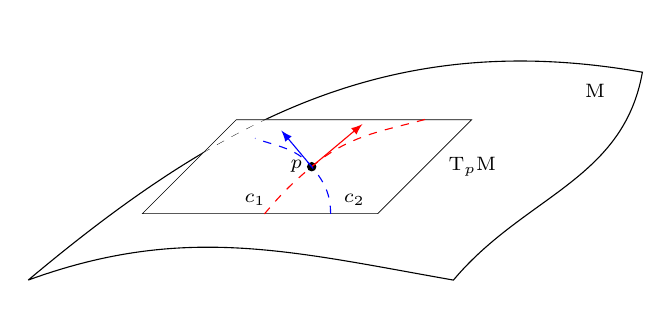
\begin{tikzpicture}[scale=1.2]
	\tikzstyle{every node}=[font=\scriptsize]
	
	\draw (1,2.8) to[out=40,in=170] (7.5,5) node at (7,4.8) {$\mathrm{M}$} to[out=-100,in=50]  (5.5,2.8) to[out=170,in=20] (1,2.8);
	
	\begin{scope}[shift={(0,0)},scale=1]
	\clip (2.2,3.5)-- (4.7,3.5) -- (5.7,4.5) -- (3.2,4.5) -- cycle;
	\draw [draw=black, fill=white] (2.2,3.5)-- (4.7,3.5) -- (5.7,4.5) -- (3.2,4.5) -- cycle;
	\draw [ultra thin, dashed] (1,2.8) to[out=40,in=170] (7.5,5) node at (7,4.8) {$\mathrm{M}$} to[out=-100,in=50]  (5.5,2.8) to[out=170,in=20] (1,2.8);
	
	\end{scope}
	\fill [black] (4,4) circle (0.05cm) node [left] {$p$};
	\node at (5.7,4) {$\mathrm{T}_p\mathrm{M}$};
	
	\draw [thin, dashed, color=red] (3.5,3.5) to[out=50,in=-140] (4,4) to[out=40,in=-165] (5.2,4.5);
	\begin{scope}[shift={(4,4)},scale=1]
	\draw [-latex, color=red] (0,0)-- (40:0.7cm);
	\end{scope}
	\node at (3.4,3.65) {$c_1$};
	
	\draw [thin, dashed, color=blue] (4.2,3.5) to[out=90,in=-50] (4,4) to[out=130,in=-20] (3.4,4.3);
	\begin{scope}[shift={(4,4)},scale=1]
	\draw [-latex, color=blue] (0,0)-- (130:0.5cm);
	\end{scope}
	\node at (4.45,3.65) {$c_2$};
	
	
	
	
	
	
	
	
	\end{tikzpicture}
	\label{fig:tangent}
	\caption{Tangent space $\mT_p\mM$ where $c_1\nsim c_2$.}
\end{figure}


It can be proven that (for a fixed atlas $\varphi$ about $p$) the following map is a linear isomorphism between $\mT_p\mM$ and $\mR^n$:
$$\begin{aligned} \Theta_\varphi:\ \mT_p&\mM &\to\ &\mR^n,\\
							&\dot{c}&\mapsto \ & (\varphi\circ c)'(0).
   \end{aligned} $$
Hence we can think about $\mT_p\mM$ as being a copy of $\mR^n$ attached to the point $p$ on the manifold.\\
For reasons that we will see later, we denote the basis of $\mT_p\mM$ as
\[\left\{  \parz{ }{x^1}(p),\dots,\parz{ }{x^n}(p)    \right\}.\]

Collecting all the tangent spaces we have the \textbf{tangent bundle} of a manifold $\mM$, defined as the disjoint union of them:
\[ \mT\mM=\bigsqcup_{p\in\mM} \mT_p\mM=\bigcup_{p\in\mM} \{p\}\times \mT_p\mM. \]

\begin{definition}
	Let $f:\mM\to\mathrm{N}$ be a differentiable map between manifolds and let $p\in \mM$. The \textbf{differential} of $f$ at $p$ is the linear map
	\[\dd_p f:\mT_p\mM\to\mT_{f(p)}\mathrm{N},\quad \dot{c}\mapsto (f\circ c)\dot\ \cong (f\circ c)'(0).   \]
	The \textbf{differential} of $f$ is the map $\dd f:\mT\mM\to\mT\mathrm{N}$ such that $\dd f|_{\mT_p\mM}=\dd_p f$.
\end{definition}


\begin{figure}[h]
	\centering
	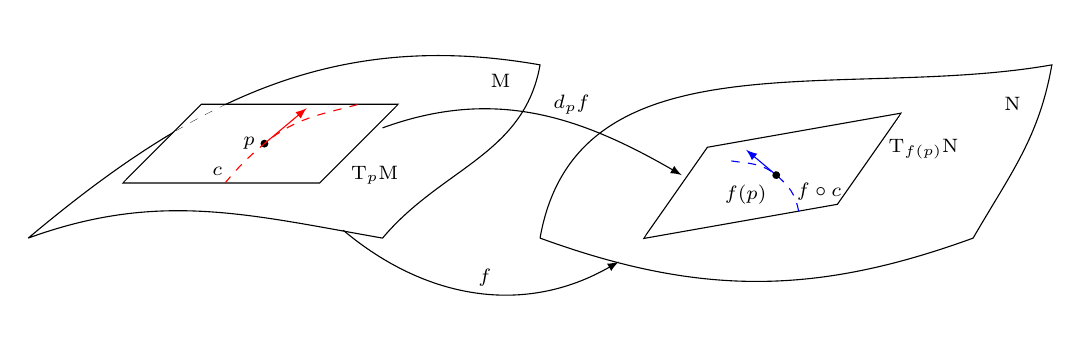
\begin{tikzpicture}[scale=1]
	\tikzstyle{every node}=[font=\scriptsize]
	
	\draw (1,2.8) to[out=40,in=170] (7.5,5) node at (7,4.8) {$\mathrm{M}$} to[out=-100,in=50]  (5.5,2.8) to[out=170,in=20] (1,2.8);
	
	\begin{scope}[shift={(0,0)},scale=1]
	\clip (2.15,3.45)-- (4.75,3.45) -- (5.75,4.55) -- (3.15,4.55) -- cycle;
	\draw [draw=black, fill=white] (2.2,3.5)-- (4.7,3.5) -- (5.7,4.5) -- (3.2,4.5) -- cycle;
	\draw [ultra thin, dashed] (1,2.8) to[out=40,in=170] (7.5,5) node at (7,4.8) {$\mathrm{M}$} to[out=-100,in=50]  (5.5,2.8) to[out=170,in=20] (1,2.8);
	
	\end{scope}
	
	\fill [black] (4,4) circle (0.05cm) node [left] {$p$};
	\node at (5.4,3.6) {$\mathrm{T}_p\mathrm{M}$};
	
	\draw [thin, dashed, color=red] (3.5,3.5) to[out=50,in=-140] (4,4) to[out=40,in=-165] (5.2,4.5);
	\begin{scope}[shift={(4,4)},scale=1]
	\draw [-latex, color=red] (0,0)-- (40:0.7cm);
	\end{scope}
	\node at (3.4,3.65) {$c$};
	
	\begin{scope}[shift={(6.5,0)},scale=1]
	\draw (1,2.8) to[out=80,in=190] (7.5,5) node at (7,4.5) {$\mathrm{N}$} to[out=-100,in=60]  (6.5,2.8) to[out=200,in=-20] (1,2.8);
	\end{scope}
	
	\begin{scope}[shift={(6.5,-0.4)},scale=1, rotate around={10:(4,4)}]
	\node at (5.9,4) {$\mathrm{T}_{f(p)}\mathrm{N}$};
	\clip (2.15,3.45)-- (4.75,3.45) -- (5.75,4.55) -- (3.15,4.55) -- cycle;
	\draw [draw=black, fill=white] (2.2,3.5)-- (4.7,3.5) -- (5.7,4.5) -- (3.2,4.5) -- cycle;
	%\draw [ultra thin, dashed] (1,2.8) to[out=40,in=170] (7.5,5) node at (7,4.8) {$\mathrm{M}$} to[out=-100,in=50]  (5.5,2.8) to[out=170,in=20] (1,2.8);
	
	\draw [thin, dashed, color=blue] (4.2,3.5) to[out=90,in=-50] (4,4) to[out=130,in=-20] (3.4,4.3);
	
	
	\begin{scope}[shift={(4,4)},scale=1]
	\draw [-latex, color=blue] (0,0)-- (130:0.5cm);
	\end{scope}
	\node at (4.5,3.7) {$f\circ c$};
	
	\fill [black] (4,4) circle (0.05cm) node [below left] {$f(p)$};
	
	\end{scope}
	
	\draw [-latex] (5,2.9) to[out=-40,in=-150] (8.5,2.5);
	\node at (6.8,2.3) {$f$};
	\draw [-latex] (5.5,4.2) to[out=20,in=150] (9.3,3.6);
	\node at (7.9,4.5) {$d_p f$};
	
	
	
	
	\end{tikzpicture}
	\label{fig:differential}
	\caption{A scheme of differential map.}
	
\end{figure}

Given a differentiable manifold $\mM$ and some chart $\{U, \varphi=(x^1,\dots,x^n)\}$ near $p$, we set $X=\dot{c}\in\mT_p\mM$. If we identify $\mT_p\mR\cong\mR$, we can interpret the differential $\dd_p f(X)$ of a function $f\in C^\infty(\mM)$ at a point $p$ as the \textbf{derivative} in the direction of $X$:
\[	\partial_X f(p):=\dd_p f(X).	\]
A functional which is linear and follows Leibniz's rule, such as $\partial_X:C^\infty(\mM)\to\mR$, is called a \textbf{derivation}. The set of all derivations at $p$ is denoted as $\operatorname{Der}_p$ and it is a vector space. It is clear that the map $X\in\mT_p\mM\mapsto\partial_X$ is an isomorphism between $\mT_p\mM$ and $\operatorname{Der}_p$.\\
We define the map:
\[	\parz{ }{x^i}(p):C^\infty(\mM)\to\mR,\quad f\mapsto\parz{f}{x^i}(p)=\partial_X f(p),	\]
where $X=\dot{c}$ and $c(t)=\varphi^{-1}(\varphi(p)+te_i)$ ($e_i$ is the basis vector).\\
Note that, from the definition of the differential, it holds
\[ \partial_X f(p)=(f\circ c)'(0)=\parz{(f\circ \varphi^{-1})}{x^i}(\varphi(p)),\]
which shows that the object we defined can be seen as a partial derivative in the usual sense.\\
It can be shown that the set of derivations $\{\parz{ }{x^1},\dots,\parz{ }{x^n}\}$ form a basis for $\operatorname{Der}_p$ and, due to the isomorphism, for $\mT_p\mM$. It is now clear why the generic tangent vector $X$ can be expressed as
\[	X=X^i\parz{ }{x^i},	\]
with Einstein convention on the sum.\\
From linearity we have the useful formula
\[	\partial_X f(p)=\dd_p f(X)=X^i\dd_p f\left(\parz{}{x^i}(p)\right)=X^i\parz{f}{x^i}(p).		\]

\begin{figure}
	\centering
	\[
	\begin{tikzcd}[column sep=1.5em]
	& \mT_p\mM \arrow{dr}{\Theta_p} \\
	\operatorname{Der}_p \arrow[<-]{ur}{X\mapsto \partial_X} && \mR^n
	\end{tikzcd}
	\]
	\caption{Isomorphism relations for the tangent space.}
\end{figure}






\begin{definition}
	Let $\mM$ be a manifold, we define a projection map $\pi:\mT\mM\to\mM$ such that $\pi(\mT_p\mM)=p$, and we call a \textbf{section} in the tangent bundle a map $s:\mM\to\mT\mM$ such that
	\[\pi\circ s=\operatorname{id}_\mM.\]
	The dual space of the tangent space $\mT_p\mM$ is called the \textbf{cotangent space}, denoted with $\mT^*_p\mM$, which has a basis denoted with $\{\dd x^1(p),\dots,\dd x^n(p)\}$. Similarly is defined the \textbf{cotangent bundle} $\mT^*\mM$ as the disjoint union of cotangent spaces.\\
	Sections in the tangent bundle, denoted by $C^\infty(\mM,\mT\mM)$, are called \textbf{vector fields} and sections in the cotangent bundle are called \textbf{$1$-forms}.
\end{definition}

Vector fields are expressed in terms of combinations of \[\left\{  \parz{ }{x^1},\dots,\parz{ }{x^n}    \right\}=:\left\{\partial_1,\dots,\partial_n\right\},\]
whereas $1$-forms are expressed as combination of
$$\{\dd x^1,\dots,\dd x^n\}.$$




\begin{definition}
We define the derivative in the direction of $X$ as an operator $\partial_X:C^\infty(\mM)\to C^\infty(\mM)$ such that
	\[ \partial_X f=\dd f(X), \]
for any vector field $X\in C^\infty(\mM,\mT\mM)$.
\end{definition}
It follows immediately that Leibniz's rule holds: $\ds \partial_X (f\cdot g)=g\,\partial_Xf +f\,\partial_X g$, and again holds the useful formula
\[	\partial_X f=\dd f(X)=X^i\dd f(\partial_i)=X^i\parz{f}{x^i}.	\]

\begin{oss}
	Given two vector fields $X,Y\in C^\infty(\mM,\mT\mM)$, there is a unique vector field $[X,Y]\in C^\infty(\mM,\mT\mM)$ such that
	\[		\partial_{[X,Y]}f=\partial_X\partial_Y-\partial_Y\partial_X f \]
	for all $f\in C^\infty(\mM)$. The map $[\cdot,\cdot ]:C^\infty(\mM,\mT\mM)\times C^\infty(\mM,\mT\mM)\to C^\infty(\mM,\mT\mM)$ is called the \textbf{Lie bracket}, it is bilinear, skew-symmetric and satisfies the well known \emph{Jacobi identity}.
\end{oss}

\begin{definition}
	An \textbf{affine connection} or \textbf{covariant derivative} on a manifold $\mM$ is a bilinear map
	
	\[\begin{split}
	\nabla: C^\infty(\mM,\mT\mM)\times C^\infty(\mM,\mT\mM) & \rightarrow C^\infty(\mM,\mT\mM)\\
	(X,Y) & \mapsto \nabla_X Y\,,
	\end{split} \]
	such that for all smooth functions $f\in C^\infty(\mM)$ and all vector fields $X,Y\in C^\infty(\mM,\mT\mM)$:
	\begin{itemize}
		\item 	$\nabla_{fX}Y= f\nabla_X Y$, i.e., $\nabla$ is $C^\infty(\mM)-$linear in the first variable;
		\item $\nabla_X (fY) = \partial_X f+ f\nabla_X Y$, i.e., $\nabla$ satisfies \emph{Leibniz rule} in the second variable.
	\end{itemize}
\label{defn:connection}
\end{definition}

The covariant derivative on the direction of the basis vector fields $\left\{\partial_1,\dots,\partial_n\right\}$ is indicated
\[	\nabla_{j}:=\nabla_{\partial_j}.	\]



We are now ready to introduce metric structures on manifolds.

\section{Lorentzian Manifolds}

We start in the simple case of \textbf{Minkowski spacetime}.

\begin{definition}
	Let $V$ be an $n$-dimensional vector space. A \textbf{Lorentzian scalar product} is a nondegenerate symmetric bilinear form $\left\langle\cdot,\cdot\right\rangle$ with signature $(-+\dots +)$, i.e. such that one can find a basis $\{e_1,\dots, e_n\}$ such that
	\[	\left\langle e_1,e_1 \right\rangle=-1,\quad \left\langle e_i,e_j \right\rangle=1\ \text{  if } i=j=2,\dots,n\ \text{ and }\left\langle e_i,e_j \right\rangle=0\text{ otherwise}.	\]
	\end{definition}
The \textbf{Minkowski product} $\scalar{x}{y}_0$, defined by the formula (with Einstein convention)
\[	\scalar{x}{y}_0=\eta_{ik}x^iy^k=-x_1\,y_1+x_2\,y_2+\cdots+x_n\,y_n,	\] with $\eta:=\operatorname{diag}(-1,1,\dots,1,1)$ is the simplest (and the only) example of Lorentzian scalar product on $\mR^n$. The $n$-dimensional Minkowski space, denoted by $\mathbb{M}^n$ is simply $\mR^n$ equipped with Minkowski product.
	\begin{figure}[h]
		\centering
		\begin{tikzpicture}[scale=1.2]
		\tikzstyle{every node}=[font=\scriptsize]
		\draw [white,postaction={decorate,decoration={text along path,text align=center,text={|\scriptsize|lightlike}}}] (-1,1.3) to [bend right=60]  (1,1.3);
		
		\begin{scope}
		\clip (-2,2.5)-- (2,2.5) -- (-2,-2.5) -- (2,-2.5) -- cycle;
		\draw [dashed] (-1,1.2) to [bend right=60]  (1,1.2);
		\draw [dashed] (-1,-0.55) to [bend right=60]  (1,-0.55);
		\end{scope}
		
		
		
		\draw [white,postaction={decorate,decoration={text along path,text align=center,text={|\scriptsize|lightlike} }}] (-1,-0.5) to [bend right=50]  (1,-0.5);
		
		
		\draw [ultra thin, -latex] (-3,-2.5) -- (-3,2.5) node [below right]{$t$};
		\draw (2,2.5)-- (-2,-2.5);
		\draw (-2,2.5)-- (2,-2.5);
		\draw (0,2.5) ellipse (2 and 0.3);
		
		\draw (2,-2.5) arc[x radius=2, y radius=0.3, start angle=0, end angle=-180];
		\draw [dashed] (2,-2.5) arc[x radius=2, y radius=0.3, start angle=0, end angle=180];
		
		
		\fill [black] (0,0) circle (0.05cm) node at (-0.1,0) [left] {$0$};
		\node at (2,1.9) {$I_+(0)$};
		\node at (2,-1.9) {$I_-(0)$};
		\node at (0,1.8) {timelike};
		\node at (0,-1.8) {timelike};
		\node at (-1.5,0) {spacelike};
		\node at (1.5,0) {spacelike};
		
		
		
		\end{tikzpicture}
		
		\label{fig:mink}
		\caption{Minkowski time orientation.}
	\end{figure}
	
\begin{definition}We call the \textbf{negative square length} of a vector $X\in V$ the quantity
	\[\gamma(X)=-\norm{X}^2:=-\scalar{X}{X}. \]
	A vector $X\in V\setminus\{0\}$ is called
\begin{itemize}
	\item  \textbf{timelike} if $\gamma(X)>0$,
	\item \textbf{lightlike} if $\gamma(X)=0$,
	\item \textbf{spacelike} if $\gamma(X)<0$ or $X=0$,
	\item \textbf{causal} if it is timelike or lightlike.
	\end{itemize}
	\end{definition}
	This definition will mostly be used for tangent vectors, in case $V$ is the tangent space of a Lorentzian manifold at some point.\\
	

	
	
	For $n\geq 2$ the set of timelike vectors $I(0)$ consists of two connected components. A \textbf{time orientation} is the choice of one of these two components. We name our choice $I_+(0)$ and call its elements \textbf{future-directed}.\\

	\begin{definition}	We put
	\begin{itemize}
		\item $J_+(0):=\overline{I_+(0)}$ (elements are called \textbf{future-directed}),
		\item $C_+(0):=\partial I_+(0)$ (upper \textbf{light cone}),
		\item $I_-(0):=-I_+(0)$, $J_-(0):=-J_+(0)$ (elements are called \textbf{past-directed}),
		\item $C_-(0):=-C_+(0)$ (lower \textbf{light cone}).
	\end{itemize}
	\end{definition}

	


\begin{definition}
	A \textbf{metric} $g$ on a manifold $\mM$ is given by a scalar product on each tangent space $$g:\mT_p\mM\times\mT_p\mM\to\mR$$ which depends smoothly on the base point $p$. We call it a \textbf{Riemannian metric} if the scalar product is pointwise positive definite, and \textbf{Lorentzian metric} if it is a Lorentzian scalar product.\\
	A pair $(\mM,g)$, where $\mM$ is a manifold and $g$ is a Lorentzian (Riemannian) metric is called a \textbf{Lorentzian (Riemannian) manifold}.
\end{definition}
The request of smooth dependence on $p$ may be specified as follows: given any chart $\{U,\varphi=(x^1,\dots,x^n)\}$ about $p$, the functions $g_{ij}:\varphi(U)\to\mR$ defined by $g_{ij}=g(\parz{ }{x^i},\parz{ }{x^j})$, for any $i,j=1,\dots,n$ should be differentiable. W.r.t. these coordinates one writes
\[ g=\sum_{i,j} g_{ij}\,\dd x_i\otimes \dd x_j=\sum_{i,j}g_{ij}\,\dd x_i\, \dd x_j. \]

The scalar product of two tangent vectors $v,w\in\mT_p\mM$, with coordinate chart $\varphi=(x^1,\dots x^n)$, such that $v=v^i\parz{ }{x^i}$, $w=w^j\parz{ }{x^j}$ then is
\[ \langle v,w\rangle=g_{ij}(\varphi(p))v^iw^j.   \]
When the choice of the chart is clear we will often write, with abuse of notation $g_{ij}(p):=g_{ij}(\varphi(p))$. We will indicate $g^{ij}:=(g^{-1})_{ij}$.\\

From now on $\mM$ will always indicate a \textbf{Lorentzian manifold}.

\begin{definition}
		A vector field $X\in C^\infty (\mM,\mT\mM)$ is called timelike, spacelike, lightlike or causal, if $X (p)$ is timelike, spacelike, lightlike or causal, respectively, at every point $p\in\mM$.\\
		
		A differentiable curve $c : I\to\mM$ is called timelike, lightlike,
		spacelike, causal, future-directed or past-directed if $\dot{c}(t)\in\mT_{c(t)}\mM$ is, for all $t\in I$, timelike, lightlike, spacelike, causal,
		future-directed or past-directed, respectively.\\
		
		A Lorentzian manifold $\mM$ is called \textbf{time-oriented} of there exists a timelike vector field on $\mM$. If a manifold is time-oriented, we refer to it as \textbf{spacetime}.
\end{definition}


\begin{figure}[h]
\centering
	\begin{subfigure}{.5\textwidth}

	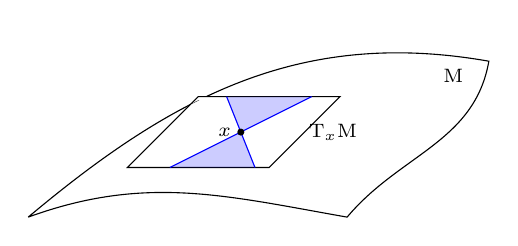
\begin{tikzpicture}[scale=0.9]
	\tikzstyle{every node}=[font=\scriptsize]
	
	\draw (1,2.8) to[out=40,in=170] (7.5,5) node at (7,4.8) {$\mathrm{M}$} to[out=-100,in=50]  (5.5,2.8) to[out=170,in=20] (1,2.8);
	
	\begin{scope}[shift={(0,0)},scale=1]
	\clip (2.2,3.4)-- (4.7,3.4) -- (5.7,4.6) -- (3.2,4.6) -- cycle;
	\draw [draw=black, thin, fill=white] (2.4,3.5)-- (4.4,3.5) -- (5.4,4.5) -- (3.4,4.5) -- cycle;
	\draw [ultra thin, dashed] (1,2.8) to[out=40,in=170] (7.5,5) node at (7,4.8) {$\mathrm{M}$} to[out=-100,in=50]  (5.5,2.8) to[out=170,in=20] (1,2.8);
	
	\draw [thin, color=blue, fill=blue, fill opacity=0.2] (3,3.5) -- (4,4) -- (4.2,3.5) ;
	
	\draw [thin, color=blue, fill=blue, fill opacity=0.2] (3.8,4.5) -- (4,4) -- (5,4.5);
	
	%\draw [thin, color=blue, fill=blue, fill opacity=0.2] (3,3.5) -- (5,4.5)-- (3.8,4.5) -- (4.2,3.5) -- (3.8,4.5);
	
	
	\end{scope}
	\fill [black] (4,4) circle (0.05cm) node [left] {$x$};
	\node at (5.3,4) {$\mathrm{T}_x\mathrm{M}$};
	
	\end{tikzpicture}
	\caption{A time-oriented tangent space.}
	\end{subfigure}

	\begin{subfigure}{.5\textwidth}

			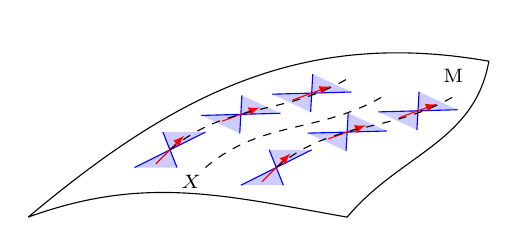
\begin{tikzpicture}[scale=0.9]
		\tikzstyle{every node}=[font=\scriptsize]
		
		\draw (1,2.8) to[out=40,in=170] (7.5,5) node at (7,4.8) {$\mathrm{M}$} to[out=-100,in=50]  (5.5,2.8) to[out=170,in=20] (1,2.8);
		
	
	\begin{scope}[shift={(-0.5,0.25)},scale=1]
	
	
	\begin{scope}[shift={(1.5,1.5)},scale=0.5]
	\clip (2.2,3.4)-- (4.7,3.4) -- (5.7,4.6) -- (3.2,4.6) -- cycle;
	\draw [thin, color=blue, fill=blue, fill opacity=0.2] (3,3.5) -- (4,4) -- (4.2,3.5) ;
	\draw [thin, color=blue, fill=blue, fill opacity=0.2] (3.8,4.5) -- (4,4) -- (5,4.5);
	\begin{scope}[shift={(4,4)},scale=1]
	\draw [-latex, color=red] (-0.4,-0.4)-- (0.4,0.4);
	\end{scope}
	
	\end{scope}
	
	\begin{scope}[shift={(2.5,2)},scale=0.5, rotate around={-25:(4,4)}]
	\clip (2.2,3.4)-- (4.7,3.4) -- (5.7,4.6) -- (3.2,4.6) -- cycle;
	\draw [thin, color=blue, fill=blue, fill opacity=0.2] (3,3.5) -- (4,4) -- (4.2,3.5) ;
	\draw [thin, color=blue, fill=blue, fill opacity=0.2] (3.8,4.5) -- (4,4) -- (5,4.5);
	\begin{scope}[shift={(4,4)},scale=1]
	\draw [-latex, color=red] (-0.4,-0.4)-- (0.4,0.4);
	\end{scope}
	\end{scope}
	
	\begin{scope}[shift={(3.5,2.3)},scale=0.5, rotate around={-25:(4,4)}]
	\clip (2.2,3.4)-- (4.7,3.4) -- (5.7,4.6) -- (3.2,4.6) -- cycle;
	\draw [thin, color=blue, fill=blue, fill opacity=0.2] (3,3.5) -- (4,4) -- (4.2,3.5) ;
	\draw [thin, color=blue, fill=blue, fill opacity=0.2] (3.8,4.5) -- (4,4) -- (5,4.5);
	\begin{scope}[shift={(4,4)},scale=1]
	\draw [-latex, color=red] (-0.4,-0.4)-- (0.4,0.4);
	\end{scope}
	\end{scope}
	
	\draw [ dashed, color=black] (3.5,3.5) to[out=40,in=-150] (6,4.5);
	\end{scope}
	
	\begin{scope}[shift={(1,0)},scale=1]
	
	
	\begin{scope}[shift={(1.5,1.5)},scale=0.5]
	\clip (2.2,3.4)-- (4.7,3.4) -- (5.7,4.6) -- (3.2,4.6) -- cycle;
	\draw [thin, color=blue, fill=blue, fill opacity=0.2] (3,3.5) -- (4,4) -- (4.2,3.5) ;
	\draw [thin, color=blue, fill=blue, fill opacity=0.2] (3.8,4.5) -- (4,4) -- (5,4.5);
	\begin{scope}[shift={(4,4)},scale=1]
	\draw [-latex, color=red] (-0.4,-0.4)-- (0.4,0.4);
	\end{scope}
	
	\end{scope}
	
	\begin{scope}[shift={(2.5,2)},scale=0.5, rotate around={-25:(4,4)}]
	\clip (2.2,3.4)-- (4.7,3.4) -- (5.7,4.6) -- (3.2,4.6) -- cycle;
	\draw [thin, color=blue, fill=blue, fill opacity=0.2] (3,3.5) -- (4,4) -- (4.2,3.5) ;
	\draw [thin, color=blue, fill=blue, fill opacity=0.2] (3.8,4.5) -- (4,4) -- (5,4.5);
	\begin{scope}[shift={(4,4)},scale=1]
	\draw [-latex, color=red] (-0.4,-0.4)-- (0.4,0.4);
	\end{scope}
	\end{scope}
	
	\begin{scope}[shift={(3.5,2.3)},scale=0.5, rotate around={-25:(4,4)}]
	\clip (2.2,3.4)-- (4.7,3.4) -- (5.7,4.6) -- (3.2,4.6) -- cycle;
	\draw [thin, color=blue, fill=blue, fill opacity=0.2] (3,3.5) -- (4,4) -- (4.2,3.5) ;
	\draw [thin, color=blue, fill=blue, fill opacity=0.2] (3.8,4.5) -- (4,4) -- (5,4.5);
	\begin{scope}[shift={(4,4)},scale=1]
	\draw [-latex, color=red] (-0.4,-0.4)-- (0.4,0.4);
	\end{scope}
	\end{scope}
	
	\draw [ dashed, color=black] (3.5,3.5) to[out=40,in=-150] (6,4.5);
	\end{scope}
	\draw [ dashed, color=black] (3.5,3.5) to[out=40,in=-150] (6,4.5);
	\node at (3.3,3.3) {$X$};
		
		\end{tikzpicture}
	\caption{A time-oriented manifold together with field lines of a timelike vector field $X$.}
	\end{subfigure}
	\label{fig:timemanif}
	\caption{Time orientations.}
\end{figure}

The \textbf{causality relations} on $\mM$ are defined as follows. Let $p,q\in\mM$,
\begin{itemize}
	\item $p\ll q$ iff there is a future-directed timelike curve from $p$ to $q$,
	\item $p< q$ iff there is a future-directed causal curve from $p$ to $q$,
	\item $p\le q$ iff $p<q$ or $p=q$.
\end{itemize}
The causality relation "$<$" is a strict weak ordering and the relation "$\le$" make the manifold a partially ordered set.\\

\begin{definition}
	The \textbf{chronological future} of a point $x\in\mM$ is the set $I_+^M(x)$ of points that can be reached by future-directed \textsl{timelike} curves, i.e.
	\[		I_+^M(x)=\{y\in\mM\ |\ x<y\}.	\]
	The \textbf{causal future} $J_+^M(x)$ of a point $x\in\mM$ is the set of points that can be reached by future-directed \textsl{causal} curves from $x$, i.e.,
	\[	J_+^M(x)=\{y\in\mM\ |\ x\le y\}.	\]
	Given a subset $A\subset \mM$ the \textbf{chronological future} and the \textbf{causal future} of $A$ are respectively
	\[	I_+^M(A)=\bigcup_{x\in A}I_+^M(x),\qquad J_+^M(A)=\bigcup_{x\in A}J_+^M(x).	\]
	In a similar way, one defines the \textbf{chronological} and \textbf{causal pasts} of a point $x$ or a subset $A \subset \mM$ by replacing \textsl{future-directed curves} by \textsl{past directed curves}. They are denoted by $I_-^M (x), I_-^M (A), J_-^M (x)$, and $J_-^M (A)$, respectively. We will also use the notation $J^M (A) := J_-^M (A) \cup J_+^M (A)$.
\end{definition}

\begin{definition}
	A connected open subset $\Omega\subset\mM$ of a spacetime is called \textbf{causally compatible} if for any point $x\in\Omega$ holds
	\[	J_{\pm}^{\Omega}(x)=J_{\pm}^{\mM}(x)\cap\Omega,		\]
	where it is clear that the inclusion "$\subset$" always holds.
\end{definition}


\begin{figure}[h]
	\centering\begin{tikzpicture}
	\tikzstyle{every node}=[font=\scriptsize]
	\draw [black] plot [smooth cycle] coordinates { (0,0) (1,1) (3,0) (1.5,-1)};
	\node at (1.5,0) {$A$};
	\begin{scope}[shift={(2.7,-0.42)},scale=1]
	\draw [color=red] (0,0) -- (45:3cm);
	\end{scope}
	
	\begin{scope}[shift={(2.9,0.13)},scale=1]
	\draw [color=blue] (0,0) -- (-45:2.5cm);
	\end{scope}
	
	\begin{scope}[shift={(0.25,-0.33)},scale=1]
	\draw [color=red] (0,0) -- (135:3cm);
	\end{scope}
	
	
	\begin{scope}[shift={(0.3,0.58)},scale=1]
	\draw [color=blue] (0,0) -- (-135:3cm);
	\end{scope}
	
	\node at (1.5,1.7) {$J_+^M(A)$};
	\node at (1.5,-1.7) {$J_-^M(A)$};
	%\draw [ultra thin, -latex] (-2.5,-2.5) -- (-2.5,2.5) node [below right]{$t$};
	\end{tikzpicture}
	\label{fig:causalfuturepast}
	\caption{Causal future $J_+^M$ and causal past $J_-^M$ of a subset $A\subset\mM$. }
\end{figure}


We now can introduce the concept of \textbf{geodesics} and \textbf{exponential map}.

\begin{definition}
	Let $c : [a,b]\to \mM$ be a curve on a Lorentzian manifold $\mM$. The
	length $L[c]$ is defined by (with Einstein convention on sum)
	\[ L[c]=\int_{a}^{b} \sqrt{|g(\dot{c}(t),\dot{c}(t))|}\,d t=\int_{a}^{b} \sqrt{\left|g_{ik}(c(t)) \deri{x^i}{t}\deri{x^k}{t}\right|}\,d t,\]
	where $x^i(t):=(\varphi\circ c)^i(t)$ are the coordinates of the point $c(t)$ on a chart $\varphi$.\\
	Given $p,q\in\mM$, if $p\leq q$ we define the \textbf{time-separation} between $p$ and $q$ as
	\[\tau(p,q)=\sup\{L[c]\ |\ c \text{ is a future directed causal curve from }p\text{ to } q\} \]
	and $0$ otherwise.\\
	A \textbf{geodesic} between two points $p,q\in\mM$ such that $p\leq q$, if it exists, is a curve $c$ such that $L[c]=\tau(p,q)$, i.e. the curve of maximum time-separation.
\end{definition}
The request on the geodesics implies that (in variational sense) $\delta L[c]=0$. It can be demonstrated that the stationary problem for the functional $L[c]$ is totally equivalent to $\delta E[c]=0$ for the functional, called \textbf{energy}, defined by
\[		E[c]=\frac{1}{2}\int_{a}^{b} {|g(\dot{c}(t),\dot{c}(t))|}\,d t.	\]
Hence, the Euler-Lagrange equations for the stationarity of a functional $I[c]=\int_{a}^{b} f(t,c(t),\dot{c}(t))\, dt$ read
\[		\deri{ }{t}\left(\parz{f}{\dot{x}^i}\right)-\parz{f}{x^i}=0,	\]
if we still denote $c=(x^1,\dots,x^n)$.\\
In our case $f(t,c,\dot{c})=g(\dot{c},\dot{c})$ and the equations become in a chart $\varphi$ (with Einstein convention):
\[  \frac{\dd^2 x^i}{\dd t^2}-\Gamma_{jk}^i\deri{x^j}{t}\deri{x^k}{t}=0,	\]
where $\Gamma_{jk}^i\in C^\infty (U\subset\mM)$ are the \textbf{Christoffel symbols}, functions defined in the chart $\varphi=(\xi^1,\dots,\xi^n)$ as
\[	\Gamma_{jk}^i=\frac12 \sum_l g^{il} \left(
\frac{\partial g_{lj}}{\partial \xi^k} 
+\frac{\partial g_{lk}}{\partial \xi^j}
-\frac{\partial g_{jk}}{\partial \xi^l}
\right).	\]

\begin{definition}
	A connection $\nabla$ on a manifold $\mM$ with a metric $g$ is said to be a \textbf{metric connection} if for all $X,Y,Z\in C^\infty (\mM,\mT\mM)$ holds the following \emph{Leibniz rule}:
	\[		\partial_X\,g(Y,Z)=g(\nabla_X Y, Z)+g(Y,\nabla_X Z).	\]
	The unique metric connection which is also torsion-free, i.e.,
	\[		T:=\nabla_X Y-\nabla_Y X-[X,Y]=0,	\]
	is called the \textbf{Levi-Civita connection}. 
\end{definition}

Another way to define \textbf{geodesics} is to say a geodesic between two points $p,q$ on a manifold $\mM$ with the Levi-Civita connection $\nabla$ is the curve $c$ which links $p$ and $q$ such that parallel transport along the curve preserves the tangent vector to the curve, i.e.
\begin{equation}
	\nabla_{\dot{c}(t)}\dot{c}(t)=0\quad \text{for all } t\in [a,b].
	\label{eq:LCgeodesic}
\end{equation}
More precisely, in order to define the covariant derivative of $\displaystyle \dot {c }$ it is necessary first to extend $\displaystyle \dot {c }$ to a smooth vector field in an open set containing the image of the curve, but it can be shown that the derivative is independent of the choice of the extension.\\

\begin{oss}
	We can express the Christoffel symbols in terms of the Levi-Civita connection:
	\begin{equation}
			\nabla_{j}\partial_k=\Gamma_{jk}^i \partial_i
			\label{eq:LCchrist}
	\end{equation}
in a local chart $\varphi=(x^1,\dots,x^n)$.
\end{oss}

\begin{prop}
	Let $\nabla$ be a connection over a manifold $\mM$ and $X,Y\in C^\infty(\mM,\mT\mM)$ be vector fields. It holds
	\[	\nabla_X Y=\left(X^j\partial_jY^k+X^jY^i\Gamma_{ij}^k\right)\partial_k,		\]
	in particular
	\[	(\nabla_j Y)^i=\partial_jY^i+Y^i\Gamma_{ij}^k		\]
\end{prop}
\Proof From the rules of definition (\ref{defn:connection}) holds:
\[	\nabla_X Y=\nabla_{X^je_j}Y^i e_i=X^j\partial_j Y^i e_i=X^jY^i\nabla_j e_i+X^j e_i\partial_j Y^i=		\]
\[	=X^jY^i\Gamma_{ij}^k e_k+(X^j\partial_jY^k) e_k		\]


\begin{prop}
	Let us consider $p\in\mM$ and a tangent vector $\xi\in \mT_p\mM$. Then there exists $\epsilon>0$ and precisely one geodesic $$c_\xi:[0,\epsilon]\to\mM$$ such that $c_\xi(0)=p$ and $\dot c_\xi(0)=\xi$.
\end{prop}

\begin{definition}
	In the conditions of the proposition above, if we put
	\[		\mathcal{D}_p=\{	\xi\in\mT_p\mM\ |\ c_\xi \text{ is defined on } [0,1]	\}\subset \mT_p\mM,	\]
	the \textbf{exponential map} at point $p$ is defined as $\exp_p:\mathcal{D}_p\to\mM$ such that $\exp_p(\xi)=c_\xi(1)$.\\
	The local coordinates defined by the chart $\{U:=\exp_p(\mathcal{D}_p),\exp_p^{-1} \}$ are called \textbf{normal coordinates} centered at $p$.
\end{definition}

\begin{figure}[h]
	\centering
		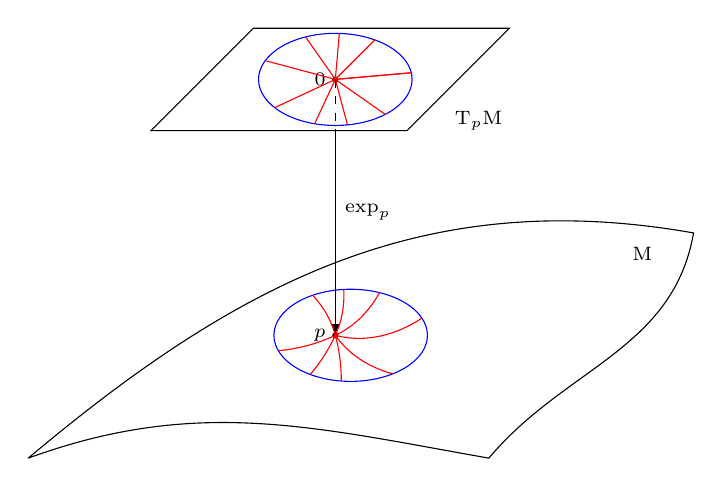
\begin{tikzpicture}[scale=1.3]
	\tikzstyle{every node}=[font=\scriptsize]
	
	\draw (1,2.8) to[out=40,in=170] (7.5,5) node at (7,4.8) {$\mathrm{M}$} to[out=-100,in=50]  (5.5,2.8) to[out=170,in=20] (1,2.8);
	
	\begin{scope}[shift={(0,2.5)},scale=1]
		\node at (5.4,3.6) {$\mathrm{T}_p\mathrm{M}$};
	%\clip (2.2,3.6)-- (4.7,3.5) -- (5.7,4.5) -- (3.2,4.5) -- cycle;
	\draw [draw=black, fill=white] (2.2,3.5)-- (4.7,3.5) -- (5.7,4.5) -- (3.2,4.5) -- cycle;
	\fill [black] (4,4) circle (0.03cm) node [left] {$0$};
	\draw [draw=blue, rotate around={0:(4,4)}] (4,4) ellipse (0.75cm and 0.45cm);
	
	\end{scope}
	
	\begin{scope}[shift={(4,6.5)},scale=1]
	\clip (0,0) ellipse (0.75cm and 0.45cm);
	\foreach \x in {0,...,9}
	\draw [thin, color=red] (0,0)-- ({5+40*\x}:2cm);
	\end{scope}
	
	
	\draw [ dashed] (4,6.5) -- (4,6);
	\draw [ -latex] (4,6) -- (4,4) node [pos=0.4, right] {$\exp_p$};
	
	
	\begin{scope}[shift={(0,0)},scale=1]
	%\clip (2.2,3.6)-- (4.7,3.5) -- (5.7,4.5) -- (3.2,4.5) -- cycle;
	\fill [black] (4,4) circle (0.03cm) node [left] {$p$};
	\draw [draw=blue, rotate around={0:(4,4)}] (4.15,4) ellipse (0.75cm and 0.45cm);
	
	\end{scope}
	
	\begin{scope}[shift={(4,4)},scale=1]
	\clip (0.15,0) ellipse (0.75cm and 0.45cm);
	\foreach \x in {0,...,4}
	\draw [thin, color=red] (0,0) to [bend right=60] ({5+40*\x}:2cm);
	\foreach \x in {4,...,6}
	\draw [thin, color=red] (0,0) to [bend left=40] ({5+40*\x}:2cm);
	\end{scope}
	
	
	\end{tikzpicture}
	\label{fig:exp}
	\caption{The exponential maps from the tangent space to the manifold.}
\end{figure}

\begin{prop}
	Il normal coordinates centered at $p\in\mM$, it holds
	\[	g_{ij}(p):=g_{ij}(\exp_p(0))=\eta_{ij},\] \[ \Gamma_{jk}^i=0 	\]
	for all indexes $i,j,k$.
\end{prop}

We are now ready to talk about \textbf{geodesically starshaped} sets.


\begin{definition}
	An open subset $\Omega\subset\mM$ is called \textbf{geodesically starshaped} with respect to a point $p\in\mM$ if there exists an open subset $\Omega'\subset\mT_p\mM$, starshaped with respect to 0, such that the exponential map
	\[	\exp_p|_{\Omega'}:\Omega'\to\Omega		\]
	is a diffeomorphism. If $\Omega$ is geodesically starshaped with respect to all of its points, one calls it \textbf{convex}.
\end{definition}

\begin{prop}
	Under the conditions of the last definition, let $\Omega\subset\mM$ be geodesically starshaped with respect to point $p\in\mM$. Then one has
	\[	I_{\pm}^\Omega(p)=\exp_p(I_{\pm}(0)\cap\Omega'),		\]
	\[	J_{\pm}^\Omega(p)=\exp_p(J_{\pm}(0)\cap\Omega').		\]
\end{prop}

\subsection{Causality and Global Hyperbolicity}



Now we introduce causal domains, because they will appear in the theory of wave equations: the local construction of fundamental solutions is always possible on causal domains, provided they are small enough.


\begin{definition}
	A domain $\Omega\subset\mM$ is called \textbf{causal} if its closure $\overline{\Omega}$ is contained in a convex domain $\Omega'$ and for any $p,q\in\overline{\Omega}$ $J_{+}^{\Omega'}(p)\cap J_{-}^{\Omega'}(q)$ is compact and contained in $\overline{\Omega}$.\\
	A subset $A\subset\mM$ is called \textbf{past-compact} (respectively \textbf{future-compact}) if, for all $p\in\mM$, $A\cap J_-^{\mM}(p)$ (respectively $A\cap J_+^{\mM}(p)$) is compact.
\end{definition}

\begin{figure}[h]
	\centering
	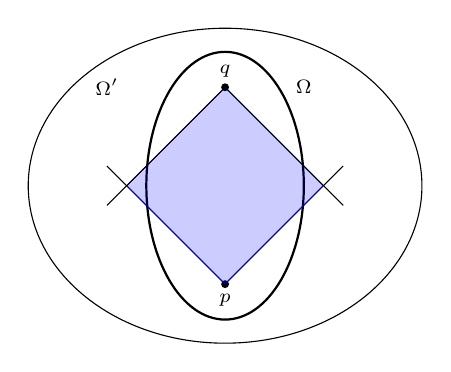
\begin{tikzpicture}
	\draw[thin] (0,0) ellipse (2.5 and 2);
	\draw[thick] (0,0) ellipse (1 and 1.7);
	\fill [black] (0,1.25) circle (0.05cm) node [above] {$q$};
	\fill [black] (0,-1.25) circle (0.05cm) node [below] {$p$};
	\begin{scope}[shift={(0,-1.25)},scale=1]
	\draw (0,0) -- (1.5,1.5);
	\draw (0,0) -- (-1.5,1.5);
	\clip (0,0) -- (1.25,1.25) -- (0,2.5) -- (-1.25,1.25) -- cycle;
	\draw [thin, color=blue, fill=blue, fill opacity=0.2] (0,0) -- (1.25,1.25) -- (0,2.5) -- (-1.25,1.25) -- cycle;
	\end{scope}
	\begin{scope}[shift={(0,1.25)},scale=1]
	\draw (0,0) -- (1.5,-1.5);
	\draw (0,0) -- (-1.5,-1.5);
	\end{scope}
	\node at (1,1.25) {$\Omega$};
	\node at (-1.5,1.25) {$\Omega'$};
	\end{tikzpicture}
	\caption{Convex, but non causal, domain}
\end{figure}

We can notice that if we look at compact spacetimes something strange happens: 

\begin{prop}
	If a spacetime $\mM$ is compact, there exists a closed timelike curve in $\mM$.
\end{prop}
In poor words, in a compact spacetimes there are timelike loops that can produce science fictional paradoxes. To avoid such unphysical and unrealistic things we require some causality conditions:
\begin{definition}
	A spacetime satisfies the \textbf{causality condition} if it does not contain any closed causal curve. A spacetime $\mM$ satisfies the \textbf{strong causality condition} if there are no almost closed causal curves, i.e. if for any $p\in\mM$ there exists a neighborhood $U$ of $p$ such that there exists no timelike curve that passes through $U$ more than once.
\end{definition}
It is clear that the strong causality condition implies the causality condition.
\begin{figure}
	\centering
	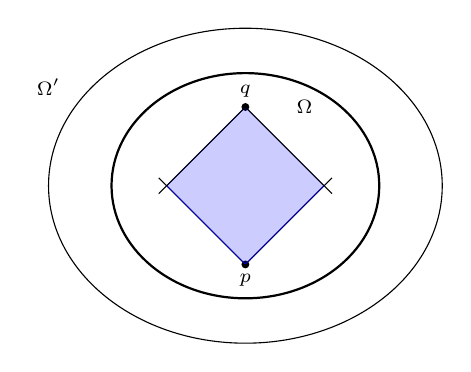
\begin{tikzpicture}
	\draw[thin] (0,0) ellipse (2.5 and 2);
	\draw[thick] (0,0) ellipse (1.7 and 1.43);
	\fill [black] (0,1) circle (0.05cm) node [above] {$q$};
	\fill [black] (0,-1) circle (0.05cm) node [below] {$p$};
	\begin{scope}[shift={(0,-1)},scale=1]
	\draw (0,0) -- (1.1,1.1);
	\draw (0,0) -- (-1.1,1.1);
	\clip (0,0) -- (1,1) -- (0,2) -- (-1,1) -- cycle;
	\draw [thin, color=blue, fill=blue, fill opacity=0.2] (0,0) -- (1,1) -- (0,2) -- (-1,1) -- cycle;
	\end{scope}
	\begin{scope}[shift={(0,1)},scale=1]
	\draw (0,0) -- (1.1,-1.1);
	\draw (0,0) -- (-1.1,-1.1);
	\end{scope}
	\node at (0.75,1) {$\Omega$};
	\node at (-2.5,1.25) {$\Omega'$};
	\end{tikzpicture}
	\caption{Causal domain}
\end{figure}
\begin{definition}
	A spacetime $\mM$ that satisfies the strong causality condition and such that for all $p,q\in\mM$ $J_+^{\mM}(p)\cap J_-^{\mM}(q)$ is compact is called \textbf{globally hyperbolic}.
\end{definition}

It can be demonstrated that in globally hyperbolic manifolds for any $p\in\mM$ and any compact set $K\subset\mM$ the sets $J_{\pm}^{\mM}(p)$ and $J_{\pm}^{\mM}(K)$ are closed.

\begin{definition}
	A subset $S$ of a connected time-oriented Lorentzian manifold $\mM$ is a \textbf{Cauchy hypersurface} if each inextendible timelike curve (i.e. no reparametrisation of the curve can be continuously extended) in $\mM$ meets $S$ at exactly one point.
\end{definition}


\begin{figure}
	\begin{subfigure}{.5\textwidth}
	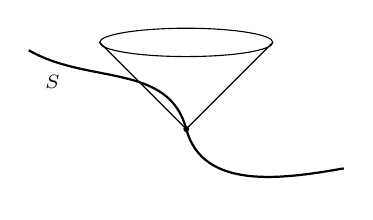
\begin{tikzpicture}
	\draw[thick] (-2,1) to[out=-30,in=105] (0,0) to[out=-75,in=190] (2,-0.5);
	\draw (0,0) -- (1.1,1.1);
	\draw (0,0) -- (-1.1,1.1);
	\draw (0,1.1) ellipse (1.1 and 0.18);
	\draw[fill=black] (0,0) circle (0.03cm);
	\node at (-1.7,0.6) {$S$};
	\end{tikzpicture}
	\caption{A non-Cauchy hypersurface}
\end{subfigure}
\begin{subfigure}{.5\textwidth}
	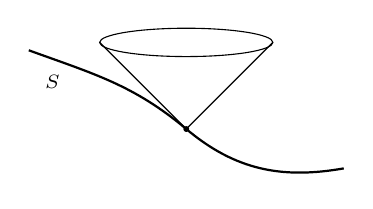
\begin{tikzpicture}
	\draw[thick] (-2,1) to[out=-20,in=140] (0,0) to[out=-40,in=190] (2,-0.5);
	\draw (0,0) -- (1.1,1.1);
	\draw (0,0) -- (-1.1,1.1);
	\draw (0,1.1) ellipse (1.1 and 0.18);
	\draw[fill=black] (0,0) circle (0.03cm);
	\node at (-1.7,0.6) {$S$};
	\end{tikzpicture}
	\caption{A Cauchy hypersurface}
\end{subfigure}
\caption{}
\end{figure}


In other words, no point of a Cauchy hypersurface is in the light cone of another point of the surface.
\begin{theorem}
	Let $\mM$ be a connected time-oriented Lorentzian manifold. Then $\mM$ is globally hyperbolic \emph{if and only if} there exists a Cauchy hypersurface in $\mM$.\\
	In such case there exists a smooth function $h:\mM\to\mR$ whose gradient is past-directed timelike at every point and all of whose level sets are spacelike Cauchy hypersurfaces.
\end{theorem}


\section{Operators and integration on manifolds}
We call $\ds\mD(\mM):= C_0^\infty(\mM)$ (the set of $C^\infty$ functions on a manifold with compact support) the space of test-functions on $\mM$. We define the integral map
\[	\int_{\mM}\cdot\ \dd\mu:\mD(\mM)\to \mC	\]
such that for any local chart $\{U,\varphi\}$ and for any $f\in\mD(U)$ holds
\[	\int_{\mM}f\,\dd\mu=\int_{\varphi(U)}(f\circ\varphi^{-1})(x)\,\mu_x\,\dd^nx,		\]
where we define \begin{equation}
	\mu_x:=|\det g(x)|^{1/2}.
\end{equation}

In this section we introduce the \textbf{generalized d'Alembert} operators. The general form of a generalized d'Alembert operator $P$ is given by
\[	P=-g^{ij}(x)\frac{\partial^2}{\partial x^i\partial x^j}+a_j(x)\parz{}{x^j}+b(x).			\]
The d'Alembert operator $\Box$ is defined for smooth functions $f$ as
\[	\Box f=-\operatorname{div}\grad f,	\]
where $\grad f$ is a vector field defined by the request that the formula $$\scalar{\grad f}{X}=\partial_X f$$ holds for any vector field $X$ and $\operatorname{div}$ is defined in the following
\begin{definition}
	The \textbf{divergence} of a vector field $Z=Z^i\partial_i$ is defined as
	\[	\operatorname{div}Z=\sum_{j}(\nabla_j Z)_j=\partial_jZ^j+\Gamma_{ij}^jZ^j.	\]
\end{definition}

\begin{prop}
	The following formula holds:
	\[	\operatorname{div}Z=\mu_x^{-1}\parz{}{x^j}\left(\mu_xZ^j\right)	\]
	and the definition of divergence is consistent with the definition of integral.
\end{prop}
\Proof Let $h\in\mD(\mM)$, using integration by parts
\[	\int_{\mM} h\cdot\operatorname{div}(Z)\dd\mu=-\int_\mM Z^j \partial_j h\,\dd\mu = -\int_\mM Z^j \partial_j h\, \mu_x\,\dd x.	\]
Now integrate by parts again, but this time in the chart geometry:
\[	-\int_\mM \partial_j h\  Z^j \mu_x\, \dd x= \int_\mM h\ \partial_j (\mu_x\, Z^j)\, \dd x = \int_\mM h\ \mu_x^{-1}\partial_j(\mu_x\ Z^j)\, \dd\mu.		\]
Since this is true for all function $h$, the formula is proved.\endproof\\

From the definition of gradient one can simply show
\[g_{ij}(\grad f)^iX^j=\partial_X f=X^j\parz{f}{x^j},\quad \grad f=g^{ij}\parz{f}{x^i}\partial_j, \]
hence holds
\[	\Box f=-\mu_x^{-1}\parz{}{x^j}\left(\mu_x\, g^{ij}\parz{f}{x^i}\right).	\]
In Minkowski space, where $g=\eta$,
\[	\Box f=-\parz{}{x^j}\left(\eta^{jj}\parz{f}{x^j}\right)=\frac{\partial^2f}{\partial t^2}-\sum_{i=1}^{n-1}\frac{\partial^2f}{\partial x_i^2}=-\partial^i\partial_if.		\]

\section{Distributions and Fourier Transform}
\large{\textbf{SECTION TO EXTEND!1!!?'?}}\\

Firstly, we recall the main concepts of the theory of distributions.
\begin{definition}
	The space of distributions over a manifold $\mM$ is defined as
	\[	\mD'(\mM)=\{u:\mD(\mM)\to\mC\text{ linear and continuous }   \}.				\]
\end{definition}



The distribution $\ds\frac{1}{x}$ is defined as
\begin{equation}
	\frac{1}{x}=\operatorname{PV}\left(\frac{1}{x}\right)-i\pi\delta(x).
\end{equation}

A particular useful formula gives
\begin{equation}
	\delta(x^2-a^2)=\frac{1}{2|a|}[\delta(x-a)+\delta(x+a)]
	\label{eq:delta1}
\end{equation}

Given a scalar product $\langle\cdot,\cdot\rangle$ on $\mR^n$, the Fourier transform $\hat{f}$ of a function $f\in L^1(\mR^n)$ is defined as
\begin{equation}
	\hat{f}(k)=\int_{\mR^n}f(x)e^{-i\langle k,x\rangle}\,\dd x
\end{equation}

We naturally extend the Fourier transform to a unitary map $L^2(\mR^n)\to L^2(\mR^n)$ and to act on tempered distributions in such a way that for $\varphi\in\mathcal{S}'(\mathcal{U})$ holds
\[	\hat{\varphi}(k)=\left(\varphi,e^{-i\langle k,x\rangle}\right).		\]
If $\varphi\in\mathcal{E}'(\mathcal{U})$, $\hat{\varphi}$ results a smooth function which extends to an entire function $\hat{\varphi}(z)$, $z\in\mathbb{C}$.\\

The inverse Fourier transform is given as $\widecheck{f}:=(2\pi)^{-n}\hat{f}(-x)$ and it holds that $f=\widecheck{\hat{f}}$.

\begin{prop}
	The Fourier transform of the distribution $\delta\in\mathcal{E}'(\mathcal{U})$ is
	\begin{equation}
		\hat{\delta}(k)=1.
	\end{equation}
\end{prop}
\Proof This is a straightforward computation:
\[\hat{\delta}(k)=(\delta(x),e^{-i\langle k,x\rangle})=e^0=1.\]\endproof

\begin{prop}
For $\varphi\in\mathcal{S}'(\mR^n)$ and for any multi-index $\alpha$ hold:
\[\hat{\partial^\alpha\varphi }(k)=(ik)^\alpha \hat{\varphi}(k)   \]
\[\hat{x^\alpha\varphi}(k)=(i\partial)^\alpha\hat{\varphi}(k).   \]
\end{prop}



